\subsection{Реализация алгоритма трилатерации, основанного на определении силового центра}

Другим вариантом реализации метода трилатерации может быть алгоритм, предложенный бельгийскими исследователями В.Пьерло, М.Ур\-бин-Шоф\-фреем и М.Ван Другенброек, которые свели проблему к решению системы линейных уравнений \cite{pierlot2011new}.

Чтобы объяснить суть метода, прежде всего, необходимо ввести понятие о так называемом \textit{силовом центре} (“power center” или “radial center”) трех окружностей – уникальной точке, обладающей равной мощностью (“power”) по отношению к этим окружностям. Мощность $P$ точки при этом может быть найдена по формуле:
\begin{equation} \label{for:power}
    P_{c,p} = (x-x_c)^2 + (y-y_c)^2 - R^2
\end{equation}
где ${x, y}$ – координаты точки, для которой вычисляется мощность, ${x_c, y_c}$ – координаты центра окружности радиуса $R$. Согласно формуле \ref{for:power}, если точка лежит на окружности, мощность равна нулю; меньше нуля в случае, когда точка находится внутри окружности и больше нуля, когда находится вне окружности.

\textit{Силовой линией }(“power line”) двух окружностей назовем такое геометрическое место точек, обладающих равной мощностью по отношению к этим окружностям. 

Она перпендикулярна прямой, соединяющей центры данных окружностей и проходит через область их взаимного пересечения (в случае наличия такового). Если рассматриваются три окружности, такие, что никакие две из них не расположены в одной точке, и центры которых не коллинеарны, то для них можно определить силовой центр – точкой пересечения силовых линий. На приведенном ниже рисунке силовой центр обозначен точкой.

\begin{figure}[ht]
    \centering
    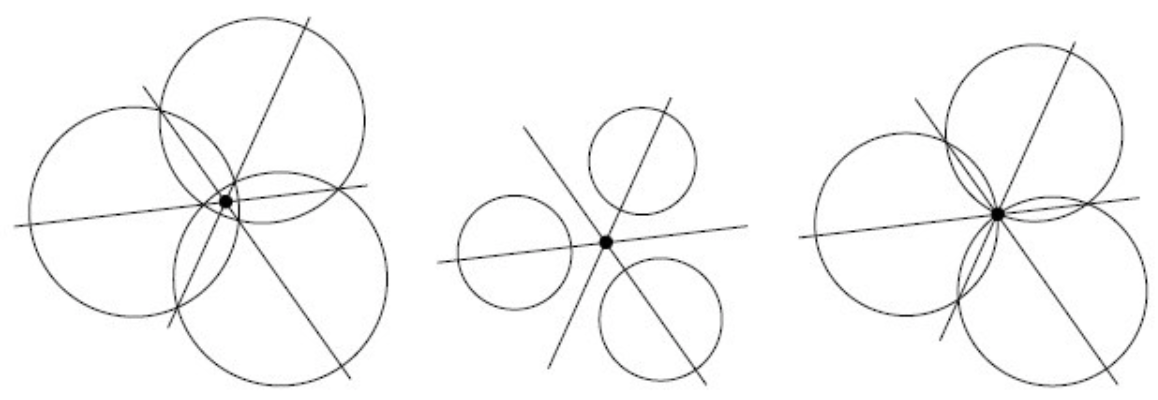
\includegraphics[width=\textwidth]{img/powerCenters}
    \caption{Определение силового центра для окружностей различных радиусов}
\end{figure}

Нахождение координаты точки пересечения двух прямых – задача, имеющая линейную сложность. В данном случае мы можем, учитывая формулу~\ref{for:power}, просто приравнять мощности.
\begin{align}
    (x-x_1)^2 + (y-y_1)^2 - R_1^2 &= (x-x_2)^2 + (y-y_2)^2 - R_2^2 \notag \\
    \Rightarrow x(x_1-x_2) + y(y_1-y_2) &= \frac{x_1^2+y_1^2-R_1^2}{2} - \frac{x_2^2+y_2^2-R_2^2}{2} \notag \\
    \Rightarrow x(x_1-x_2)+y(y_1-y_2) &= k_1 - k_2 \notag
\end{align}

Введен дополнительный коэффициент $k$, равный мощности источника относительно некоторой окружности, деленный на два:
\[
    k_n = \frac{x_n^2+y_n^2-R_n^2}{2}
\]

Наконец, чтобы определить координаты точки пересечения силовых линий, достаточно решить систему линейных уравнений:

\begin{numcases}{}
    x(x_1-x_2) + y(y_1-y_2) = k_1-k_2 \notag
    \\
    x(x_2-x_3) + y(y_2-y_3) = k_2-k_3 \label{for:system}
    \\
    x(x_3-x_1) + y(y_3-y_1) = k_3-k_1 \notag
\end{numcases}

Можно заметить, что одно из уравнений в системе может быть получено путем сложения двух других, что является, в свою очередь, доказательством пересечения трех силовых линий лишь в одной точке. Ее точные координаты можно определить по следующим формулам:
\[
    x_r = \frac{ 
	    \begin{vmatrix}
	    k_1-k_2 & y_1-y_2 \\
	    k_2-k_3 & y_2-y_3
	    \end{vmatrix}}{D},  \quad
    y_r = \frac{
    \begin{vmatrix}
   	    x_1-x_2 & k_1-k_2 \\
	    x_2-x_3 & k_2-k_3
    \end{vmatrix}}{D} 
\]

\[
    D = \begin{vmatrix}
	    x_1-x_2 & y_1-y_2 \\
	    x_2-x_3 & y_2-y_3
    \end{vmatrix} = \begin{vmatrix}
        x1 & y1 & 1 \\
        x2 & y2 & 1 \\
        x3 & y3 & 1
    \end{vmatrix}
\]

Определитель матрицы $D \neq 0$, если центры окружностей не коллинеарны, тогда же, соответственно, существует решение приведенной системы уравнений \ref{for:system}. В противном случае найти координаты пересечения прямых в явном виде нельзя.

\begin{figure}[ht]
    \centering
    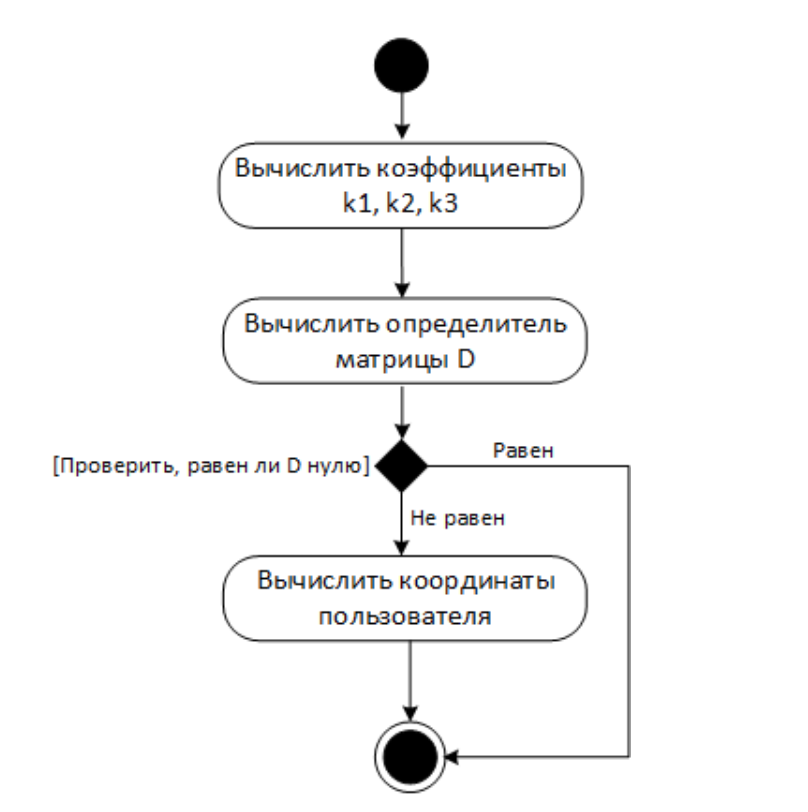
\includegraphics[scale=0.5]{img/powerCenterActivity}
    \caption{Activity-диаграмма рассматриваемого алгоритма}
\end{figure}

Исходный код, реализующий данный метод, приведен в приложении 1.